%
%%%%%%%%%%%%%%%%%%%%%%% file typeinst.tex %%%%%%%%%%%%%%%%%%%%%%%%%
%
% This is the LaTeX source for the instructions to authors using
% the LaTeX document class 'llncs.cls' for contributions to
% the Lecture Notes in Computer Sciences series.
% http://www.springer.com/lncs       Springer Heidelberg 2006/05/04
%
% It may be used as a temlpate for your own input - copy it
% to a new file with a new nam eand use it as the basis
% for your article.
%
% NB: the document class 'llncs' has its own and detailed documentation, see
% ftp://ftp.springer.de/data/pubftp/pub/tex/latex/llncs/latex2e/llncsdoc.pdf
%
%%%%%%%%%%%%%%%%%%%%%%%%%%%%%%%%%%%%%%%%%%%%%%%%%%%%%%%%%%%%%%%%%%%


\documentclass[runningheads,a4paper]{llncs}

\usepackage{amssymb}
\setcounter{tocdepth}{3}
\usepackage{graphicx}
\usepackage{amsmath}
\usepackage{booktabs}
%\usepackage{times}
\usepackage{perpage}
\usepackage{hyperref}
\MakePerPage{footnote}
\usepackage{multirow}
\usepackage{epstopdf} %converting to PDF
\usepackage{tikz}
\usetikzlibrary{arrows,patterns,automata,backgrounds,decorations,fit,petri,positioning,petri,shapes,calc}
\usepackage[caption=false]{subfig}
\usepackage{url}

\urldef{\mailsa}\path|{kerwin,andriiro,f.m.maggi,marlon.dumas}@ut.ee|
\urldef{\mailsb}\path|{dfmchiara,ghidini}@fbk.eu|
\urldef{\mailsc}\path|{ilya.verenich,m.larosa,simon.raboczi}@qut.edu.au|
\newcommand{\keywords}[1]{\par\addvspace\baselineskip
\noindent\keywordname\enspace\ignorespaces#1}

\begin{document}

\mainmatter  % start of an individual contribution

% first the title is needed
\title{Nirdizati: A Web-Based Tool for\\ Predictive Process Monitoring}

% a short form should be given in case it is too long for the running head
\authorrunning{Jorbina et al.}
\titlerunning{Nirdizati: A Web-Based Tool for Predictive Process Monitoring}

% the name(s) of the author(s) follow(s) next
%
% NB: Chinese authors should write their first names(s) in front of
% their surnames. This ensures that the names appear correctly in
% the running heads and the author index.
%
\author{Kerwin Jorbina\inst{1} \and Andrii Rozumnyi\inst{1} \and Ilya Verenich\inst{1,2}  \and Chiara Di Francescomarino\inst{3} \and  Marlon Dumas\inst{1}  \and Chiara Ghidini\inst{3}  \and Fabrizio Maria Maggi\inst{1} \and Marcello La Rosa\inst{3} \and Simon Raboczi\inst{3}}

\institute{University of Tartu, Estonia\\
\mailsa
\and Queensland University of Technology, Australia\\
\mailsc
\and FBK IRST, Trento, Italy\\
\mailsb
}

%
% NB: a more complex sample for affiliations and the mapping to the
% corresponding authors can be found in the file "llncs.dem"
% (search for the string "\mainmatter" where a contribution starts).
% "llncs.dem" accompanies the document class "llncs.cls".
%

%\toctitle{Predictive Process Monitoring Using LSTM}
%\tocauthor{Authors' Instructions}
\maketitle


\begin{abstract}
%In this paper, we present a prototype of a predictive process monitoring engine for process workers and operational managers.
%The developed solution, named \emph{Nirdizati}, is a configurable full-stack web application that supports users in selecting the preferred prediction method from the list of implemented methods and enables the continuous prediction of various performance indicators at runtime.
%The results of the predictions, as well as the real-time summary statistics about the process execution, are presented in a dashboard that offers multiple visualization options.
%The target audience of this demonstration includes process mining researchers as well as practitioners interested in exploring the potential of process monitoring.
This paper introduces Nirdizati: A web-based application for generating predictions about running cases of a business process. Nirdizati is a configurable full-stack web application that supports users in selecting and tuning prediction methods from a list of implemented algorithms and enables the continuous prediction of various performance indicators at runtime.
The tool can be used to predict the outcome, the next events, or the remaining time of each case of a process.
For example, in a lead-to-order process, Nirdizati can predict which customer leads will convert to purchase orders and when.
In a claims handling process, it can predict if a claim decision will be made on time or late.
%Based on these predictions, process workers and operational managers can act proactively to resolve or mitigate potential process performance violations.
%The target audience of this demonstration includes process mining researchers as well as practitioners interested in exploring the potential of process monitoring.
%In this paper, we present a prototype of a web-based application for predictive process monitoring that can be used by process participants and operational managers to predict the future development of a currently running process execution.
%The implemented solution, named \emph{Nirdizati}, is a configurable full-stack web application that supports users in selecting the preferred prediction methods from a list of implemented algorithms and enables the continuous prediction of various measures of interest at runtime.
The results of the predictions, as well as the real-time summary statistics about the process executions, are presented in a dashboard that offers multiple visualization options. Based on these predictions, process participants can act proactively to resolve or mitigate potential process performance violations. The target audience of this demonstration includes process mining researchers as well as practitioners interested in exploring the potential of predictive process monitoring.

\keywords{Predictive Process Monitoring, Machine Learning}
\end{abstract}


\section{Introduction} \label{sec:intro}
\emph{Predictive Process Monitoring}~\cite{PredictiveMonitoring} is an emerging paradigm based on the continuous generation of predictions about the future values of user-specified measures of interest about a currently running process execution.
%and recommendations on what activities to perform and what input data values to provide, so that the likelihood of violation of business constraints is minimized. % and violations can be avoided.
In this paradigm, a user defines the type of predictions they are interested in and a set of historical execution traces. Based on the analysis of these traces, the idea of predictive monitoring is to continuously provide the user with predictions and estimated values of the measure of interest. Such predictions generally depend both on: (i) the sequence of activities executed in a given case; and (ii) the values of data attributes after each activity execution in a case.

As an example, consider a doctor who needs to choose the most appropriate therapy for a patient. Historical data referring to patients with similar characteristics can be used to predict what therapy will be the most effective one and to advise the doctor accordingly. Meanwhile, in the context of a business process for managing loan applications, the applicant can be advised on the combinations of the loan amount and the length of loan that are the most likely to lead to acceptance of the application, given contextual information about the application and the personal data of the applicant (e.g., age, salary, etc.).

Several approaches have been proposed in the literature to tackle common predictive process monitoring tasks.
However, so far, these approaches have largely remained in the academic domain and
have not been widely applied in real-time scenarios, in which users require a continuous predictive support.

In this paper, we present Nirdizati, a pioneering open-source Web-based predictive monitoring tool, which is able to fill this gap
between research and practice, by providing business analysts with a highly configurable instrument for the configuration,
generation and analysis of different predictive models; and end-users with continuous runtime predictions.


%\vspace{-\baselineskip}
\begin{figure}[t]%[H]
	\centering
	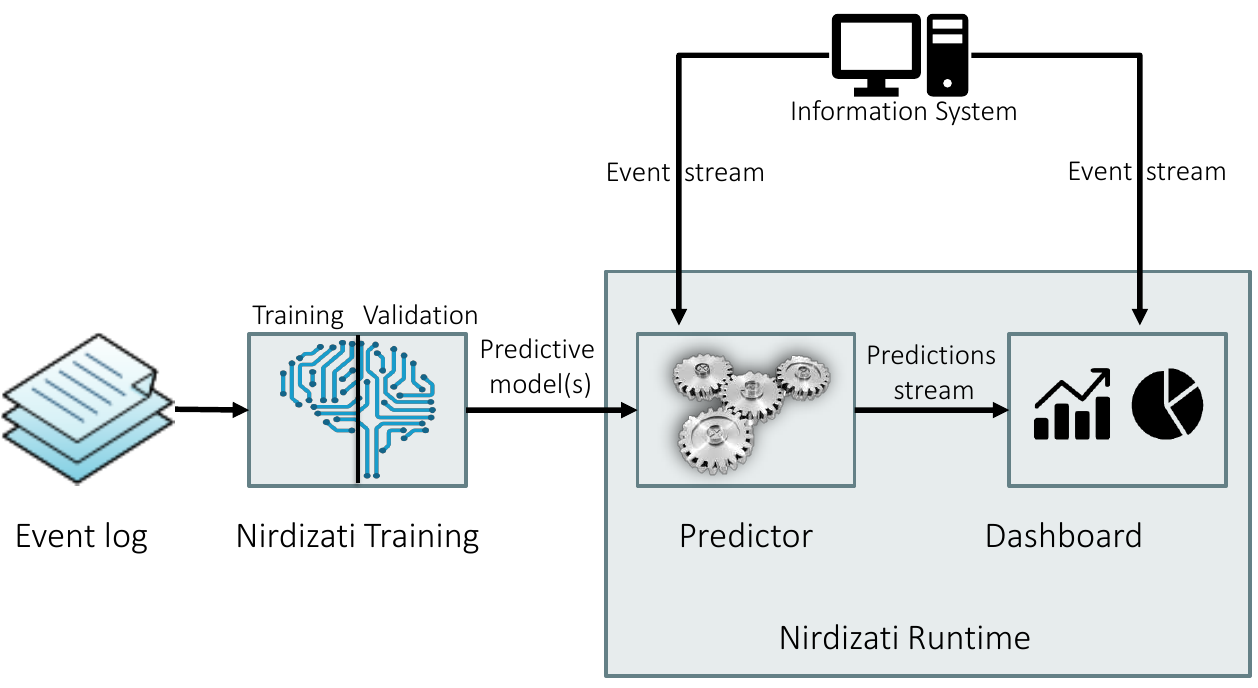
\includegraphics[width=0.7\textwidth]{img/nirdizati-overall}
	\caption{A high-level overview of Nirdizati.}
	\label{fig:nirdizati-overall}
\end{figure}
%\vspace{-\baselineskip}


Nirdizati consists of two components: \textit{Nirdizati Training} and \textit{Nirdizati Runtime} (Figure~\ref{fig:nirdizati-overall}). Nirdizati Training takes as input a business process event log and produces one or more prediction models, which can then be deployed in Nirdizati Runtime. Once a model is deployed, Nirdizati Runtime listens to a stream of events related to a business process, and produces a stream of predictions. These predictions are then visualized in a continuously updated Web dashboard.
%Nirdizati consists of two components: Nirdizati Training and Nirdizati Runtime (Figure~\ref{fig:nirdizati-overall}). Nirdizati Training takes as input a business process event log and produces a prediction model. This model can then be deployed in Nirdizati Runtime. Once a model is deployed, Nirdizati Runtime listens to a stream of events related to a business process, and produces a stream of predictions. These predictions are then visualized in a continuously updated Web dashboard.

\section{Nirdizati Training} \label{sec:training}
Nirdizati Training is the component of Nirdizati that allows users to produce predictive models later used by
Nirdizati Runtime for making predictions on streams of events. It provides several algorithms for generating
predictive models for different types of predictions and tailored to each specific dataset.
For example, it is able to build predictive models for predicting remaining time, the next activity to be
performed, whether a certain outcome will be achieved and even the overall workload per day.
%
To this aim, the training component of Nirdizati relies on two phases: a training and a validation phase.
In the former, one or more predictive models are built; in the latter, their suitability to the specific
dataset is evaluated, so as to support the user in selecting the predictive model that ensures the best results.

Nirdizati Training is composed of a front-end application, which allows users to configure the predictive models
and to assess the goodness-of-fit of the built models, and a back-end application responsible of the actual training and validation.
The back-end application is in turn composed of the four submodules shown in Figure~\ref{fig:nirdizati-training}.
A Log Manager is in charge of managing the logs. Uploading and retrieving the logs are the basic operations
of this module. The Encoder is responsible for parsing the logs, labeling them according to the desired type of prediction,
 and preparing the data for the training phase.
In the Training submodule, the encoded data are split into training and validation set used for evaluation purposes,
and the predictive models are built from the training data. Finally, the Evaluation submodule
tests the validation data against the model(s) created to get accuracy measures with respect to the ground truth,
available from the complete traces in the validation data.
The back-end application comes with a storage module for saving the uploaded logs and the built predictive models.

%First, we have the Front-end application which acts as the interface for the user to
%select settings used for prediction and to analyze the prediction results. The second
%module is the Log Manager which is responsible for managing the logs. Uploading
%and retrieving the logs are the basic operations of this module. The third module is
%the Encoder which retrieves the log from the storage, parses it and prepares the log for
%the training phase in the Predictive Module. In this part, we retrieve the encoded data,
%split it into training and test set for evaluation, and build the predictive model from the
%training data. Finally, using the test data, we test it against the model created to get its
%accuracy. The aggregation of the results are done in the Evaluation Module which is
%tasked to calculate the error of the prediction model created.

%\vspace{-\baselineskip}
\begin{figure}[t]%[H]
	\centering
	 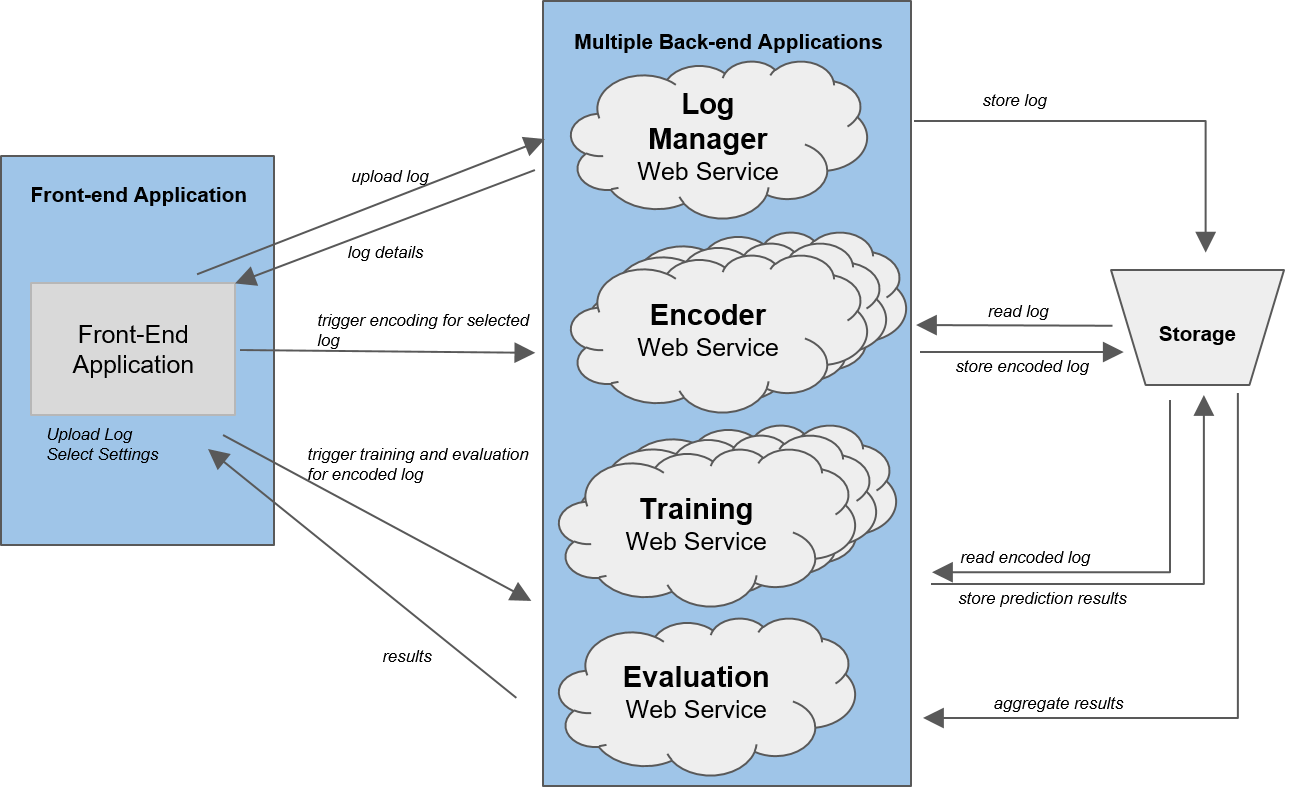
\includegraphics[width=0.7\textwidth]{img/nirdizati-training-architecture-rev}
	%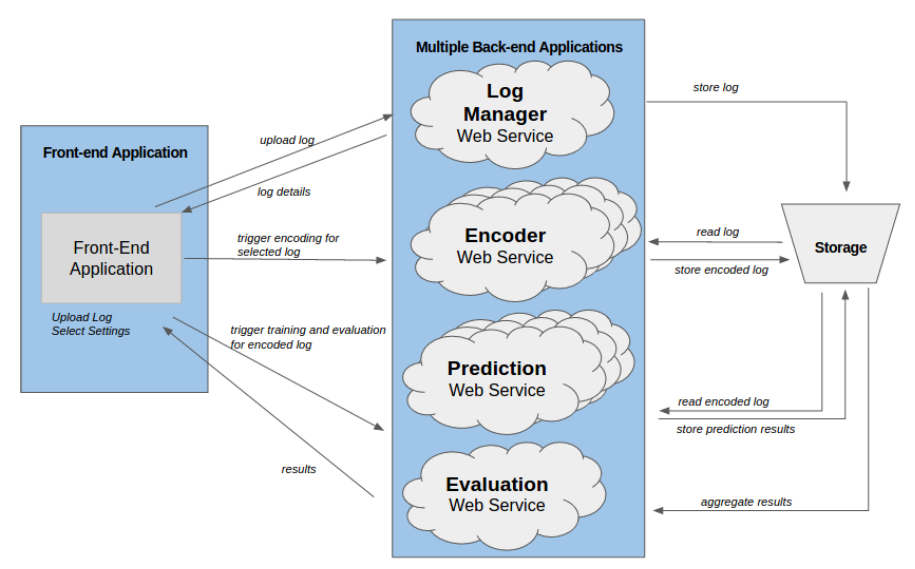
\includegraphics[width=0.7\textwidth]{img/nirdizati-training}
	\caption{A high-level overview of Nirdizati Training.}
	\label{fig:nirdizati-training}
	\vspace{-0.5\baselineskip}
\end{figure}


\section{Nirdizati Runtime} \label{sec:runtime}
Once the predictive models have been trained, they can be transferred to the Runtime component to make predictions for ongoing cases. As an input, Nirdizati Runtime takes a stream of events produced by a workflow management system (WFMS) that registers tasks performed in the organization. (Figure~\ref{fig:dfd_0}). Next, the produced stream is consumed by a web server which is responsible for storing data and further information processing.
Web server, in turn, communicates with a predictive engine which applies models obtained via Nirdizati Training for a business process and returns all the results of calculations.
After web server receives the outputs from each predictive model, it writes them to a database and updates corresponding clients.
From the user's side, the results are visualized via a dashboard-based interface which is capable of sending queries requesting various visualization options.

\begin{figure}
	\centering
	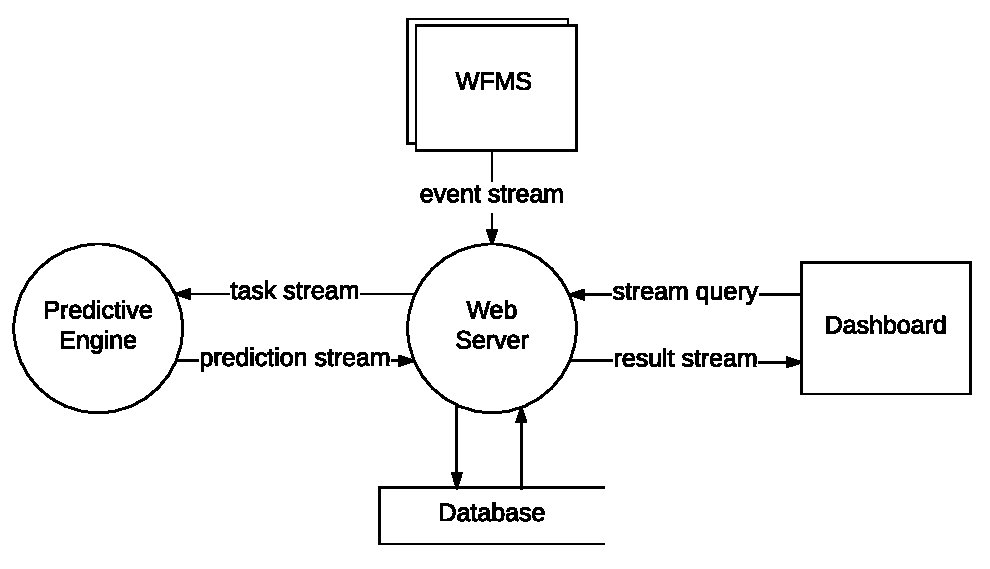
\includegraphics[width=0.7\textwidth]{img/dfd_0}
	\caption{High-level data flow diagram of Nirdizati Runtime}
	\label{fig:dfd_0}
\end{figure}
\vspace{-\baselineskip}

When a user logs into the system, they initially see a table that lists both currently ongoing cases (colored in gray) as well as completed cases (colored in green). For each case, we provide a range of summary statistics including the number of completed events in a given case, case start time and the time of the latest event completion. For ongoing cases, we also estimated their completion time and a range of other process-specific indicators, such as the probability that a customer will not accept an offer from a salesperson. For completed cases, instead, we show the actual completion time and the actual indicators.

The upper panel shows aggregated process indicators, such as the number of currently running and so far completed cases, the number of occurred events, average number of events per case and average case duration.

Nirdizati also allows monitoring multiple event streams simultaneously. The drop-down list in the top right corner allows a user to switch the stream. When a user switches to another process, all information in the dashboard is updated automatically. At the same time, each user can choose which process to monitor without interfering with others.

The Outcomes tab provides a pie chart visualization for outcomes for ongoing and completed cases. For ongoing cases, the outcome is predicted, while for completed cases, we are using the actual value. Similarly, the Case duration tab shows a histogram of case durations, while on the Case length tab, a user will find the distribution of cases by the number of events.


\begin{figure}
	\centering
	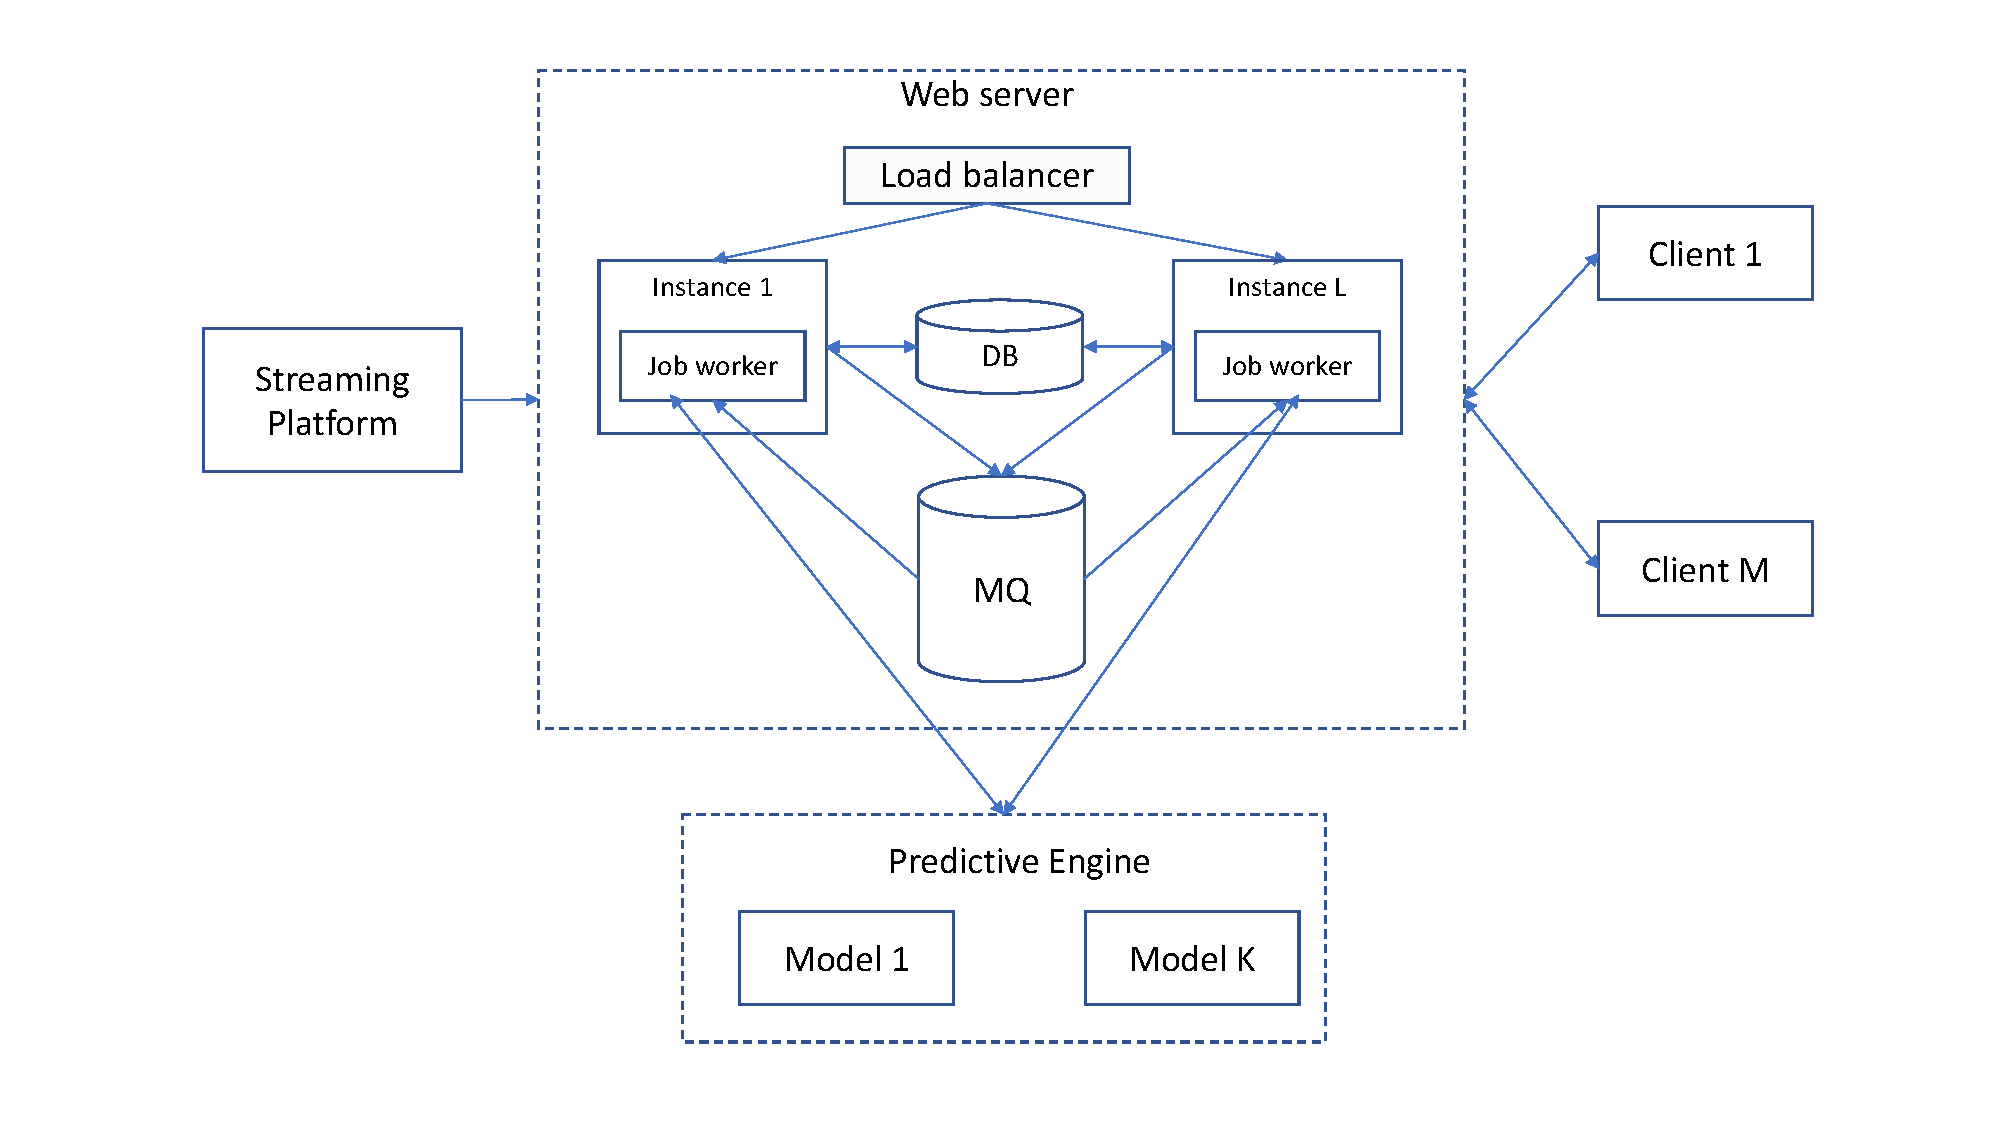
\includegraphics[width=0.9\textwidth]{img/nirdizati-runtime}
	\caption{Main view of Nirdizati Runtime}
	\label{fig:nirdizati-runtime}
	\vspace{-0.5\baselineskip}
\end{figure}
%\vspace{-\baselineskip}

Process workers and operational managers -- typical users of such system -- can set the process performance targets and subscribe to a stream of warnings and alerts generated whenever these targets are predicted to be violated. Thus, process workers will be capable of making more informed, data-driven decisions to get a better control of the process execution. This is especially beneficial for processes where process workers have more leeway to make corrective actions, for example, in a lead management process.

\section{Conclusion} \label{sec:conclusion}
The developed solution, named \emph{Nirdizati}, is a configurable full-stack web application that supports users in selecting the preferred prediction method from the list of implemented methods and enables the continuous prediction of various performance indicators at runtime.
The results of the predictions, as well as the real-time summary statistics about the process execution, are presented in a dashboard that offers multiple visualization options.

A video demo of Nirdizati can be found at \url{http://youtu.be/0nr14lX04-I}. A public release of Nirdizati Training and Nirdizati Runtime are available at \url{http://training.nirdizati.com} and \url{http://dashboard.nirdizati.com} respectively. The source code is available under the Lesser GNU Public License (LGPL) at \url{http://github.com/nirdizati}. 
\bibliographystyle{splncs03}
\bibliography{paper}

\end{document}
